% !TEX root = ../main.tex
\begin{frame}{Fiducial Cuts}
    \label{20.06::fiducial_cuts}

    \vspace{48pt}

    \begin{itemize}
        \item
            To apply fiducial cuts, we would provide \ef{$\phi$} vs. \ef{$\theta$} curves that cut events at the edges of each DC sector.

        \vspace{18pt}
        \item
            One curve would be needed for each \ef{$p$} bin, for each sector.

        \vspace{18pt}
        \item
            This would be done for each PID processed.
    \end{itemize}

    \backref{11.21::summary}
\end{frame}

\begin{frame}{Fiducial Cuts}
    \begin{center}
        \begin{figure}[t]
            \centering{
                \fbox{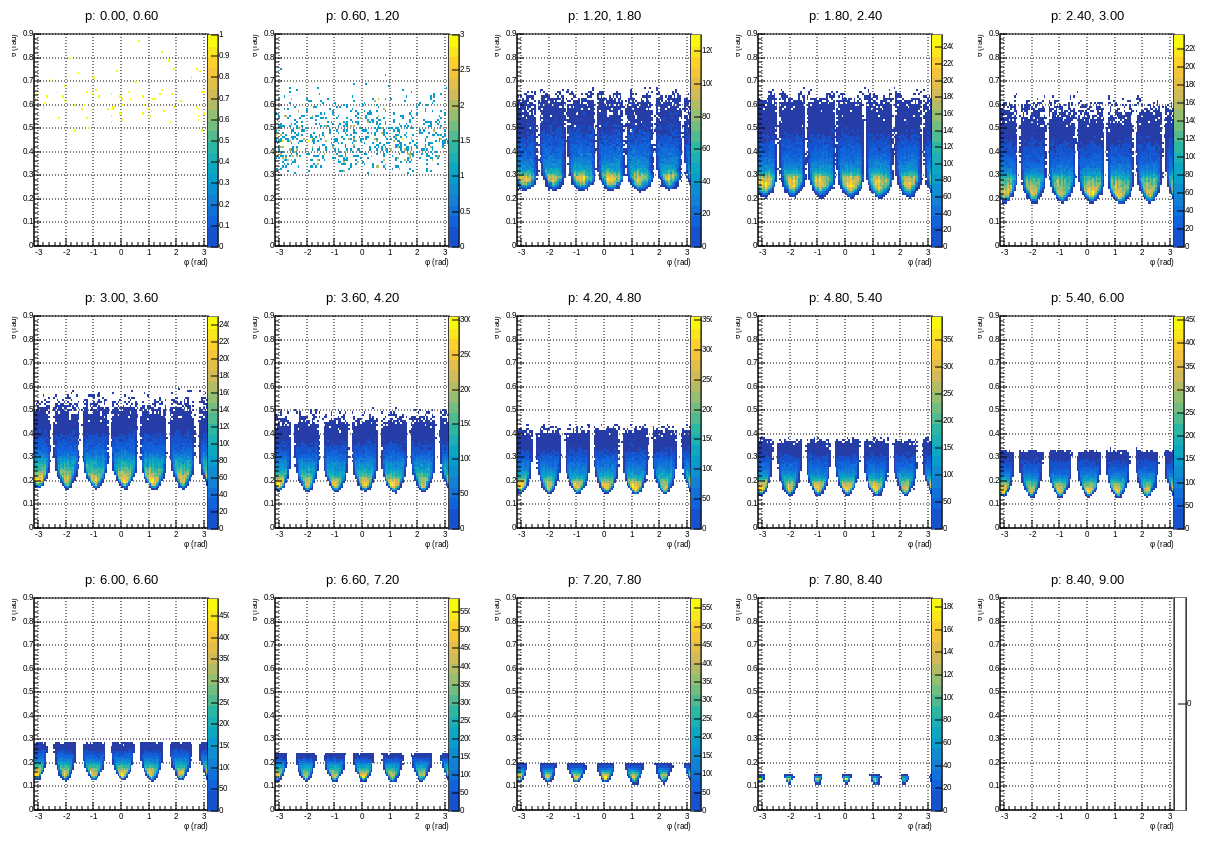
\includegraphics[width=0.72\textwidth]{06fidcuts_11.png}}
            }
        \end{figure}
        \scriptsize{\textit{
            \ef{$\phi$} vs. \ef{$\theta$} of $e^-$ detected by DC in \ef{$p$} bins. Run 12016.
        }}
    \end{center}

    \backref{11.21::summary}
\end{frame}
